\documentclass[../main.tex]{report}

\begin{document}
    \label{sec:test1}
    
\subsection{Approche probabiliste}
Soient $E_n := \left\{ k \in N^* ~|~k \leq n \right\}$ l'ensemble des entiers inférieurs ou égaux à n, $ P_n := \{k \in E_n~|~ k$ est premier$ \}$ l'ensemble des nombres premiers inférieurs ou égaux à n, et la fonction $\pi (n) := \#P_n$, le nombres de premiers inferieurs ou égaux à n.

On a vu que la fonction Li$(x) = \int_2^x \frac{dt}{\log t}$ 
donne une bonne approximation de $\pi(n)$.

Cette fonction peut être approximée par la somme de Riemann de pas contant $=1$:
\begin{equation}
\label{eq:SommeDeRiemann}
S(\frac{1}{\log x})
= \sum_{k=0}^n \frac{1}{\log(2 + k)}
= \frac{1}{\log 2} + \sum_{k=3}^n \frac{1}{\log k}
\end{equation}


La fonction $\frac{1}{\log x}$ est une fonction continue, décroissante et positive sur l'interval $\left[2, \infty \right[$. 
L'erreur entre Li$(n)$ et la fonction en escalier ci-dessus est donc bornée. 
 \[ 
\left| S(\frac{1}{\log x}) - Li(n) \right|
\leq \left| \sum_{k=2}^n \frac{1}{\log (k+1)} - \frac{1}{\log k} \right| 
 %= \left| \frac{1}{\log (n+1)} - \frac{1}{\log 2} \right|
 = \frac{1}{\log (2)} - \frac{1}{\log (n+1)}
 < \frac{1}{\log 2}
 < 2
 \]


\subsubsection{Ensembles aléatoires} 

Nous allons alors générer $k$ ensembles aléatoires $R_{k_n} \subset E_n$ de sorte que:
\[
\forall~i \in E_n, P(i \in R_{k_n}) = 
\left\{ 
    \begin{array}{cl}
         0 & \mbox{si}~i = 1 \\
         1 & \mbox{si}~i = 2 \\
         \frac{1}{\log n} & \mbox{si}~i \geq 3
    \end{array}
\right.
\]
Il est à noter deux cas particuliers:
\begin{itemize} 
    \item Le nombre 1 est exclu. En effet, $\frac{1}{\log 1}$ n'est pas défini. Par définition, $1$ n'est pas un nombre premier.
    \item Le nombre 2 est inclu par défaut. En effet, $P(2 \in R_{k_n}) = \frac{1}{\log 2} > 1$. De plus, le nombre 2 est par définition, un nombre premier.
\end{itemize}


Nous allons aussi introduire la fonction $\sigma_k(n) := \# R_{k_n}$. Cette fonction mesure la taille de l'ensemble aléatoire.\newline
$\sigma_k(n)$ est donc une valeur aléatoire strictement inférieure à $n$ dont l'espérance est donnée par la formule suivante:
\begin{equation}
\label{eq:esperance}
E[\sigma_k(n)] = 0 + 1 + \frac{1}{\log 3} + ... + \frac{1}{\log n}
= 1 + \sum_{k=3}^{n} \frac{1}{\log k}
\end{equation}

On observe alors que l'erreur entre l'espérance de $\sigma_k(n)$ et la somme de Riemann (\ref{eq:SommeDeRiemann}) est constante, égale à
$\frac{1}{\log 2}- 1 < 1$.

Les ensembles aléatoires générés de cette manière suivront donc une distribution similaire a Li$(x)$, et donc à $\pi(x)$
(voir figures \ref{fig:comparison_sigma_prob} et \ref{fig:prob_sample}).

\begin{figure}[H]
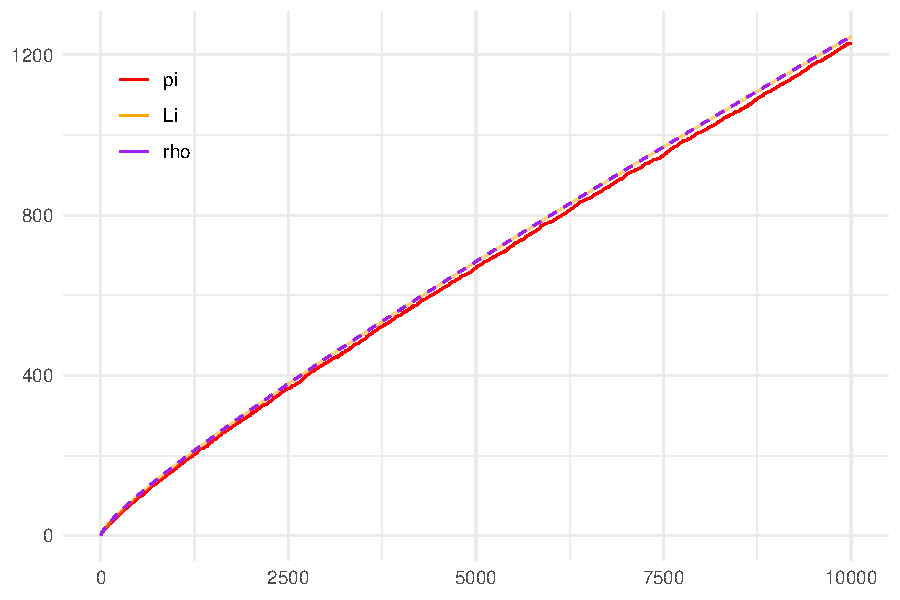
\includegraphics[width=\textwidth]{comparison_sigma_prob}

\caption{Graphes des fonctions $\pi$, Li and $\sigma$. On observe que Li et $\sigma$ sont superposées.}
\label{fig:comparison_sigma_prob}
\end{figure}

\begin{figure}[H]
	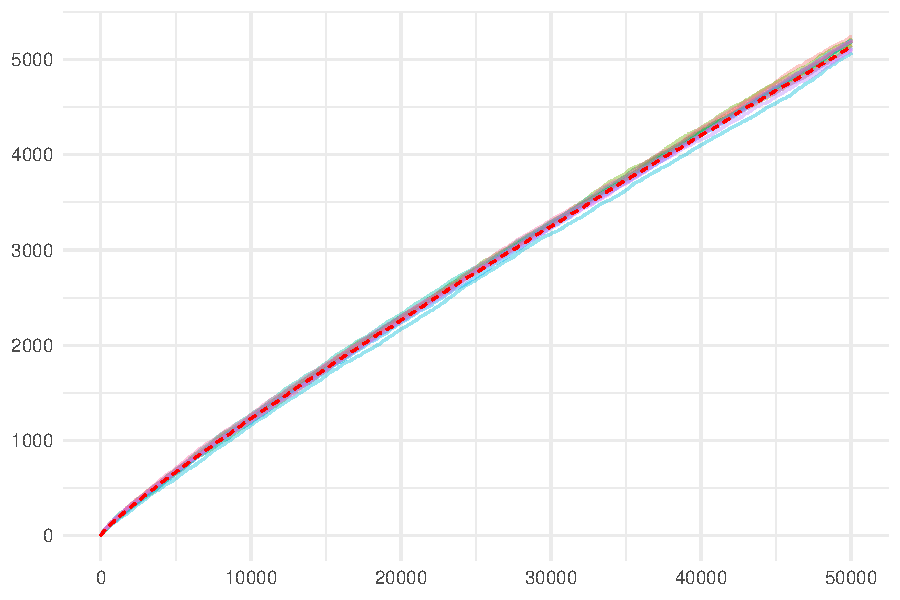
\includegraphics[width=\textwidth]{prob_sample1}
	\caption{graphes des fonctions $\sigma_k$ pour $k \leq 25$ (25 premiers ensembles) et $\pi$}
	\label{fig:prob_sample}
\end{figure}
\end{document}